\section{Góc lượng giác}

\subsection{Đề 1 }
\Opensolutionfile{ans}[ans/ans1]
\caulc
%%%==============EX_1============%%%
\begin{ex} %[1D1N1-2]
	Góc có số đo $\dfrac{\pi}{9}$ đổi sang độ là
	\choice
	{$15^{\circ}$}
	{$18^{\circ}$}
	{\True $20^{\circ}$}
	{$25^{\circ}$}
	\loigiai{
		Áp dụng công thức đổi rad sang độ $n=\dfrac{\alpha \cdot  180}{\pi}$.
		Ta có $n=\dfrac{\pi}{9} \cdot  \dfrac{180^{\circ}}{\pi}=20^{\circ}.
		$
	}
\end{ex}

%%%==============EX_2============%%%
\begin{ex}%[1D1N1-2]
	Đổi số đo góc $105^{\circ}$ sang rađian bằng
	\choice
	{$\dfrac{5\pi}{12}$}
	{\True $\dfrac{7\pi}{12}$}
	{$\dfrac{9\pi}{12}$}
	{$\dfrac{5\pi}{8}$}
	\loigiai{
		\[105^{\circ}=\dfrac{105^{\circ}\cdot \pi}{180^{\circ}}=\dfrac{7\pi}{12}.
		\]
	}
\end{ex}

%%%==============EX_3============%%%
\begin{ex}%[1D1H1-4]
	Trên đường tròn bán kính bằng $5$, cho một cung tròn có độ dài bằng $ 10$. Số đo rađian của cung tròn đó là
	\choice
	{\True $2$}
	{$3$}
	{$1$}
	{$4$}
	\loigiai{
		Ta có công thức tính độ dài của một cung tròn là $l=R\cdot \alpha \Rightarrow \alpha=\dfrac{l}{R}=\dfrac{10}{5}=2$ rad.
	}
\end{ex}

%%%==============EX_4============%%%
\begin{ex}%[1D1N1-4]
	Một đường tròn có bán kính $R=10$ cm. Độ dài cung $40^{\circ}$ trên đường tròn gần bằng:
	\choice
	{\True $7$ cm}
	{$9$ cm}
	{$11$ cm}
	{$13$ cm}
	\loigiai{
		Độ dài của cung $40^{\circ}$ trên đường tròn được tính bằng công thức $\dfrac{\pi \cdot a^{\circ}}{180} \cdot R=\dfrac{\pi}{180} \cdot 40 \cdot 10\approx 7$ cm.
	}
\end{ex}

%%%==============EX_5============%%%
\begin{ex} %[1D1H1-4]
	Cho đường tròn có bán kính bằng $9$(cm). Tìm số đo (theo radian) của cung có độ dài $3\pi$ (cm).
	\choice
	{\True $\dfrac{\pi}{3}$}
	{$\dfrac{2\pi}{3}$}
	{$\dfrac{\pi}{4}$}
	{$\dfrac{\pi}{6}$}
	\loigiai{
		\[l=R\alpha \Rightarrow \alpha=\dfrac{l}{R}=\dfrac{3\pi}{9}=\dfrac{\pi}{3}.
		\]
	}
\end{ex}
%%%==============EX_6============%%%
\begin{ex}%[1D1H1-4]
	Một bánh xe có $72$ răng. Số đo góc mà bánh xe đã quay được khi di chuyển $10$ răng là
	\choice
	{$30^\circ$}
	{$40^\circ$}
	{\True $50^\circ$}
	{$60^\circ$}
	\loigiai{
		1 bánh răng tương ứng với $\dfrac{360^\circ}{72}=5^\circ \Rightarrow$ $10$ bánh răng là $50^\circ$.
	}
\end{ex}

%%%==============EX_7============%%%
\begin{ex}%[1D1H1-4]
	Một đường tròn có bán kính $15$ cm. Tìm độ dài cung tròn có góc ở tâm bằng $30{^\circ}$ là
	\choice
	{\True $\dfrac{5\pi}{2}$}
	{$\dfrac{\pi}{3}$}
	{$\dfrac{2\pi}{5}$}
	{$\dfrac{5\pi}{3}$}
	\loigiai{
		Cung tròn có góc ở tâm bằng $30{^\circ}$ nên số đo của cung tròn bằng $n {^\circ}=30{^\circ}$. Khi đó độ dài của cũng tròn là $l=\dfrac{\pi \cdot R \cdot n {^\circ}}{180 {^\circ}}=\dfrac{\pi \cdot 15 \cdot 30{^\circ}}{180 {^\circ}}=\dfrac{5\pi}{2}$.
	}
\end{ex}

%%%==============EX_8============%%%
\begin{ex}%[1D1V1-6]
	Một đồng hồ treo tường có kim giờ dài $10{,}57$ cm. Trong $30$ phút mũi kim giờ vạch lên cung tròn có độ dài bằng bao nhiêu?
	\choice
	{\True $\dfrac{1057}{1200} \pi$ (cm)}
	{$\dfrac{1057}{2400} \pi$ (cm)}
	{$\dfrac{1057}{600} \pi$ (cm)}
	{$\dfrac{1057}{4800} \pi$ (cm)}
	\loigiai{
		Trong $1$ giờ mũi kim giờ vạch lên $1$ cung có số đo là $\dfrac{2\pi}{12}=\dfrac{\pi}{6}$ nên trong $30$ phút kim giờ vạch lên $1$ cung có số đo là $\dfrac{1}{12} \pi$.
		
		Vậy độ dài cung tròn mà mũi kim giờ vạch là $l=R\alpha=10{,}57\times \dfrac{\pi}{12}=\dfrac{1057}{1200} \pi$
	}
\end{ex}
%%%==============EX_9============%%%
\begin{ex}%[1D1H1-5]
	Góc nào trong các góc sau có điểm biểu diễn là $M\left(-\dfrac{\sqrt{3}}{2};-\dfrac{1}{2} \right)$?
	\choice
	{$-\dfrac{\pi}{3}+k2\pi \left(k\in \mathbb{Z}\right)$}
	{\True $\dfrac{7\pi}{6}+k2\pi \left(k\in \mathbb{Z}\right)$}
	{$\dfrac{2\pi}{3}+k2\pi \left(k\in \mathbb{Z}\right)$}
	{$-\dfrac{\pi}{6}+k2\pi \left(k\in \mathbb{Z}\right)$}
	\loigiai{
		Ta có $M\left(-\dfrac{\sqrt{3}}{2};-\dfrac{1}{2} \right)$ nên $M$ thuộc góc phần tư thứ ba.\\
		Gọi $H$ là hình chiếu của $M$ trên $Ox$.\\
		Khi đó $\cos \widehat{MOH}=\dfrac{OH}{OM}=\dfrac{\dfrac{\sqrt{3}}{2}}{1}=\dfrac{\sqrt{3}}{2} \Rightarrow \widehat{MOH}=\dfrac{\pi}{6}$.\\
		Vậy góc có điểm biểu diễn là $M\left(-\dfrac{\sqrt{3}}{2};-\dfrac{1}{2} \right)$ có số đo $\dfrac{\pi}{6}+\pi+k2\pi=\dfrac{7\pi}{6}+k2\pi \, \left(k\in \mathbb{Z}\right)$.
	}
\end{ex}
%%%==============EX_10============%%%
\begin{ex} %[1D1V1-5]
	Biết một góc lượng giác $\left(Ou,Ov\right)$ có số đo là $\dfrac{2021\pi}{3}$, số đo của góc hình học $uOv$ là
	\choice
	{$\dfrac{2\pi}{3}$}
	{\True $\dfrac{\pi}{3}$}
	{$\dfrac{\pi}{6}$}
	{$\dfrac{-\pi}{3}$}
	\loigiai{
		\begin{itemize}
			\item Khi $Ou,Ov$ đối nhau thì một góc lượng giác $\left(Ou,Ov\right)$ có số đo là $\pi$ rad và góc hình học $uOv$ cũng có số đo là $\pi$ rad.
			\item  Khi $Ou,Ov$ không đối nhau thì số đo góc hình học $uOv$ là $\beta$ rad $\left(0\le \beta < \pi \right)$ và góc lượng giác $\left(Ou,Ov\right)$ có số đo là $\beta+k2\pi$ hoặc $-\beta+k2\pi$ với $k\in \mathbb{Z}$, tức là
			sđ$\left(Ou,Ov\right)=\alpha+k2\pi$, với $\left|\alpha \right|=\beta$ và $k\in \mathbb{Z}$.
			\item  Ta có sđ$\left(Ou,Ov\right)=\dfrac{2021\pi}{3}=\dfrac{-\pi}{3}+674\pi=\dfrac{-\pi}{3}+337\cdot 2\pi$.
		\end{itemize}
		Vậy góc lượng giác $\left(Ou,Ov\right)$ có số đo bằng $\dfrac{2021\pi}{3}$, thì số đo góc hình học $uOv$ là $\dfrac{\pi}{3}$.
	}
\end{ex}
%%%==============EX_11============%%%
\begin{ex}%[1D1N1-4]
	Một đường tròn có bán kính $30$ cm. Tính độ dài của cung tròn trên đường tròn đó có số đo $2{,}5$.
	\choice
	{$7{,}5$ cm}
	{$0{,}83$ cm}
	{\True $75$ cm}
	{$12$ cm}
	\loigiai{
		$R=30$, $\alpha=2{,}5$ rad $\Rightarrow$ Độ dài l của cung tròn là $l=R\alpha=30\cdot 2{,}5=75$ cm.
	}
\end{ex}

%%%==============EX_12============%%%
\begin{ex}%[1D1V1-6]
	Một bánh xe quay theo chiều dương được $5$ vòng trong $8$ giây. Trong $3$ giây bánh xe quay được một góc lượng giác có số đo là bao nhiêu
	\choice
	{$\dfrac{3}{4} \pi$}
	{$\dfrac{48}{5} \pi$}
	{\True $\dfrac{15}{4} \pi$}
	{$\dfrac{5}{6} \pi$}
	\loigiai{
		Trong $3$ giây bánh xe quay được $\dfrac{5\cdot 3}{8}=\dfrac{15}{8}$ vòng.\\
		Bánh xe quay $1$ vòng được một góc là $2\pi$.\\
		Vậy bánh xe quay $\dfrac{15}{8}$ vòng được $1$ góc là $2\pi \cdot \dfrac{15}{8}=\dfrac{15}{4} \pi$.
	}
\end{ex}
\Closesolutionfile{ans}
\indapan{6}{ans/ans1}

\cauds
\Opensolutionfile{ans}[ans/ans1-ds]

%%%==============EX_1============%%%
\begin{ex}%[1D1N1-2]
	Đổi số đo của các góc sang radian. Khi đó các mệnh đề sau \textbf{ĐÚNG} hay \textbf{SAI}?
	\choiceTF
	{\True $30 ^{\circ}=\dfrac{\pi}{6}$ rad}
	{\True $\left(\dfrac{15}{\pi} \right) ^{\circ}=\dfrac{1}{12}$ rad}
	{\True $132 ^{\circ}=\dfrac{11\pi}{15}$ rad}
	{$-495 ^{\circ}=-\dfrac{13\pi}{4}$ rad}
	\loigiai{
		\begin{itemchoice}
			\itemch $30 ^{\circ}=\dfrac{30\pi}{180} $ rad $=\dfrac{\pi}{6} $ rad.
			\itemch 	$\left(\dfrac{15}{\pi} \right) ^{\circ}=\dfrac{\dfrac{15}{\pi} \pi}{180} $ rad$ =\dfrac{1}{12} $ rad.
			\itemch 	$132 ^{\circ}=\dfrac{132\pi}{180} $ rad $=\dfrac{11\pi}{15} $ rad.
			\itemch 	$-495 ^{\circ}=\dfrac{-495\pi}{180} $ rad $=-\dfrac{11\pi}{4} $ rad.
		\end{itemchoice}
	}
\end{ex}


%%%==============EX_2============%%%
\begin{ex}%[1D1H1-4]
	\immini{Các mệnh đề dưới đây \textbf{ĐÚNG} hay \textbf{SAI} ?
		\choiceTF
		{\True $125 ^{\circ}$ là điểm $M$ thuộc góc phần tư thứ thứ II}
		{$405 ^{\circ}$ là điểm $N$ thuộc góc phần tư thứ III}
		{$\dfrac{19\pi}{3}$ là điểm $P$ thuộc góc phần tư thứ II}
		{\True $-\dfrac{13\pi}{6}$ là điểm $Q$ thuộc góc phần tư thứ IV}}{
		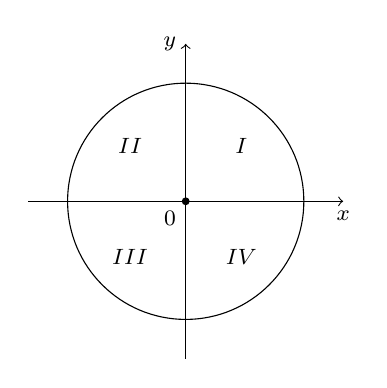
\begin{tikzpicture}[font=\footnotesize]
			\draw[->] (180:2)--(0:2) node[below] {$x$};
			\draw[->] (-90:2)--(90:2) node[left] {$y$};
			\draw (0:0) circle (1.5);
			\fill (0:0) circle (0.05) node[below left] {$0$};
			\node at (45:1) {$I$};
			\node at (135:1) {$II$};
			\node at (225:1) {$III$};
			\node at (-45:1) {$IV$};
		\end{tikzpicture}
	}
	\loigiai{
		\begin{itemchoice}
			\itemch 	\immini{Điểm biểu diễn của góc lượng giác có số đo $125 ^{\circ}$ là điểm $M$ thuộc góc phần tư thứ thứ II của đường tròn lượng giác thoả mãn $\widehat{AOM}=125 ^{\circ}$ .}
			{
				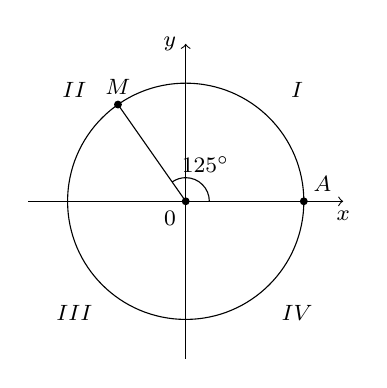
\begin{tikzpicture}[font=\footnotesize]
					\draw[->] (180:2)--(0:2) node[below] {$x$};
					\draw[->] (-90:2)--(90:2) node[left] {$y$};
					\draw (0:0) circle (1.5);
					\fill (0:0) circle (0.05) node[below left] {$0$};
					\node at (45:2) {$I$};
					\node at (135:2) {$II$};
					\node at (225:2) {$III$};
					\node at (-45:2) {$IV$};
					\fill (125:1.5) circle (0.05) node[above] {$M$};
					\fill (0:1.5) circle (0.05) node[above right] {$A$};
					\draw (0:0)--(125:1.5)  (0:0.3) arc (0:125:0.3) node[above right] {$125^\circ$};
				\end{tikzpicture}
			}
			\itemch \immini{	Ta có $405 ^{\circ}=45 ^{\circ}+360 ^{\circ}$. 
				
				Vì vậy điểm biểu diễn của góc lượng giác $405 ^{\circ}$ là điểm $N$ thuộc góc phần tư thứ $I$ của đường tròn lượng giác và thoả mãn $\widehat{AON}=45 ^{\circ}$ .}
			{
				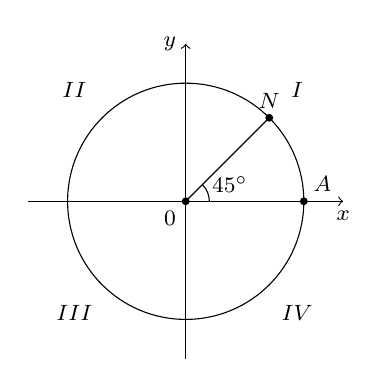
\begin{tikzpicture}[font=\footnotesize]
					\draw[->] (180:2)--(0:2) node[below] {$x$};
					\draw[->] (-90:2)--(90:2) node[left] {$y$};
					\draw (0:0) circle (1.5);
					\fill (0:0) circle (0.05) node[below left] {$0$};
					\node at (45:2) {$I$};
					\node at (135:2) {$II$};
					\node at (225:2) {$III$};
					\node at (-45:2) {$IV$};
					\fill (45:1.5) circle (0.05) node[above] {$N$};
					\fill (0:1.5) circle (0.05) node[above right] {$A$};
					\draw (0:0)--(45:1.5)  (0:0.3) arc (0:45:0.3) node[right] {$45^\circ$};
				\end{tikzpicture}
			}
			\itemch 	\immini{Ta có $\dfrac{19\pi}{3}=\dfrac{18\pi+\pi}{3}=\dfrac{\pi}{3}+3\cdot2\pi$.
				
				Vì vậy điểm biểu diễn của góc lượng giác $\dfrac{19\pi}{3}$ là điểm $P$ thuộc góc phần tư thứ $I$ của đường tròn lượng giác và thoả mãn $\widehat{AOP}=\dfrac{\pi}{3}$ .}
			{
				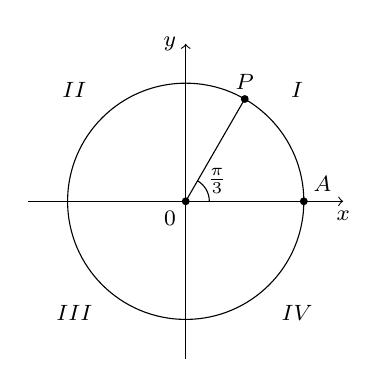
\begin{tikzpicture}[font=\footnotesize]
					\draw[->] (180:2)--(0:2) node[below] {$x$};
					\draw[->] (-90:2)--(90:2) node[left] {$y$};
					\draw (0:0) circle (1.5);
					\fill (0:0) circle (0.05) node[below left] {$0$};
					\node at (45:2) {$I$};
					\node at (135:2) {$II$};
					\node at (225:2) {$III$};
					\node at (-45:2) {$IV$};
					\fill (60:1.5) circle (0.05) node[above] {$P$};
					\fill (0:1.5) circle (0.05) node[above right] {$A$};
					\draw (0:0)--(60:1.5)  (0:0.3) arc (0:60:0.3) node[right] {$\frac{\pi}{3}$};
				\end{tikzpicture}
			}
			\itemch \immini{
				Ta có $-\dfrac{13\pi}{6}=\dfrac{-12\pi-\pi}{6}=-\dfrac{\pi}{6}-2\pi$. 
				
				Vì vậy điểm biểu diễn của góc lượng giác $-\dfrac{13\pi}{6}$ là điểm $Q$ thuộc góc phần tư thứ IV của đường tròn lượng giác và thoả mãn $\widehat{AOQ}=\dfrac{\pi}{6}$.}
			{
				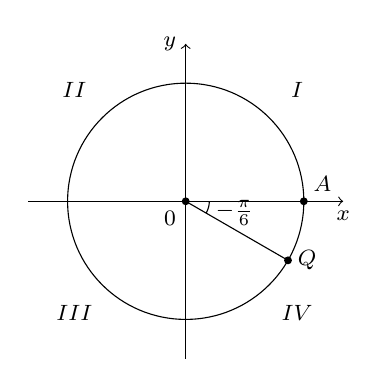
\begin{tikzpicture}[font=\footnotesize]
					\draw[->] (180:2)--(0:2) node[below] {$x$};
					\draw[->] (-90:2)--(90:2) node[left] {$y$};
					\draw (0:0) circle (1.5);
					\fill (0:0) circle (0.05) node[below left] {$0$};
					\node at (45:2) {$I$};
					\node at (135:2) {$II$};
					\node at (225:2) {$III$};
					\node at (-45:2) {$IV$};
					\fill (-30:1.5) circle (0.05) node[ right ] {$Q$};
					\fill (0:1.5) circle (0.05) node[above right] {$A$};
					\draw (0:0)--(-30:1.5)  (0:0.3) arc (0:-30:0.3) node[right] {$-\frac{\pi}{6}$};
				\end{tikzpicture}
			}
		\end{itemchoice}
	}			
\end{ex}

%%%==============EX_3============%%%
\begin{ex} %[1D1H1-4]
	Các mệnh đề sau đây \textbf{ĐÚNG} hay \textbf{SAI}?
	\choiceTF
	{\True Điểm biểu diễn của góc lượng giác có số đo $218 ^{\circ}$ là điểm $M$ thuộc góc phần tư thứ III của đường tròn lượng giác thoả mãn $\widehat{AOM}=218 ^{\circ}$}
	{Điểm biểu diễn của góc lượng giác có số đo $-405 ^{\circ}$ là điểm $N$ thuộc góc phần tư thứ IV của đường tròn lượng giác thoả mãn $\widehat{AON}=-45 ^{\circ}$}
	{\True Điểm biểu diễn của góc lượng giác có số đo $\dfrac{25\pi}{4}$ là điểm $P$ thuộc góc phần tư thứ I của đường tròn lượng giác thoả mãn $\widehat{AOP}=\dfrac{\pi}{4}$}
	{Điểm biểu diễn của góc lượng giác có số đo $\dfrac{15\pi}{2}$ là điểm $Q(0;-1)$ thuộc đường tròn lượng giác thoả mãn $\widehat{AOQ}=-\dfrac{\pi}{2}$}
	\loigiai{
		\begin{itemchoice}
			\itemch \immini{Điểm biểu diễn của góc lượng giác có số đo $218 ^{\circ}$ là điểm $M$ thuộc góc phần tư thứ III của đường tròn lượng giác thoả mãn $\widehat{AOM}=218 ^{\circ}$. 	}{
				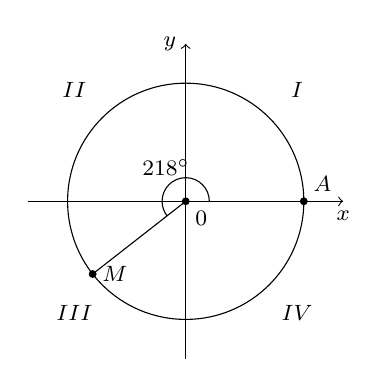
\begin{tikzpicture}[font=\footnotesize]
					\draw[->] (180:2)--(0:2) node[below] {$x$};
					\draw[->] (-90:2)--(90:2) node[left] {$y$};
					\draw (0:0) circle (1.5);
					\fill (0:0) circle (0.05) node[below right] {$0$};
					\node at (45:2) {$I$};
					\node at (135:2) {$II$};
					\node at (225:2) {$III$};
					\node at (-45:2) {$IV$};
					\fill (218:1.5) circle (0.05) node[ right ] {$M$};
					\fill (0:1.5) circle (0.05) node[above right] {$A$};
					\draw (0:0)--(218:1.5)  (0:0.3) arc (0:218:0.3);
					\node[] at (120:0.5) {$218^\circ$};
				\end{tikzpicture}
			}			
			\itemch \immini{	Ta có $-405 ^{\circ}=-45 ^{\circ}-360 ^{\circ}$.
				
				Điểm biểu diễn của góc lượng giác có số đo $-405 ^{\circ}$ là điểm $N$ thuộc góc phần tư thứ IV của đường tròn lượng giác thoả mãn $\widehat{AON}=45 ^{\circ}$.	}{
				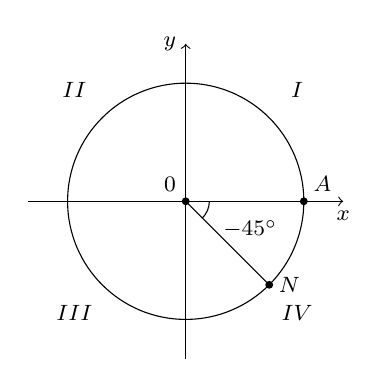
\begin{tikzpicture}[font=\footnotesize]
					\draw[->] (180:2)--(0:2) node[below] {$x$};
					\draw[->] (-90:2)--(90:2) node[left] {$y$};
					\draw (0:0) circle (1.5);
					\fill (0:0) circle (0.05) node[above left] {$0$};
					\node at (45:2) {$I$};
					\node at (135:2) {$II$};
					\node at (225:2) {$III$};
					\node at (-45:2) {$IV$};
					\fill (-45:1.5) circle (0.05) node[ right ] {$N$};
					\fill (0:1.5) circle (0.05) node[above right] {$A$};
					\draw (0:0)--(-45:1.5)  (0:0.3) arc (0:-45:0.3);
					\node[right] at (-45:0.5) {$-45^\circ$};
				\end{tikzpicture}
			}			
			\itemch  \immini{	Ta có $\dfrac{25\pi}{4}=\dfrac{\pi+24\pi}{4}=\dfrac{\pi}{4}+6\pi$.
				
				Điểm biểu diễn của góc lượng giác có số đo $\dfrac{25\pi}{4}$ là điểm $P$ thuộc góc phần tư thứ I của đường tròn lượng giác thoả mãn $\widehat{AOP}=\dfrac{\pi}{4}$.	}{
				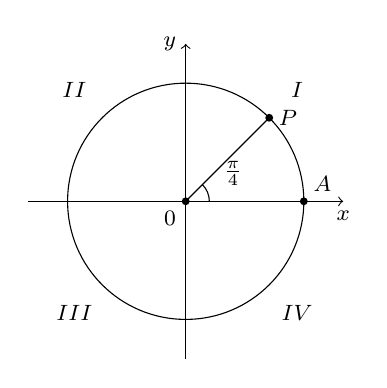
\begin{tikzpicture}[font=\footnotesize]
					\draw[->] (180:2)--(0:2) node[below] {$x$};
					\draw[->] (-90:2)--(90:2) node[left] {$y$};
					\draw (0:0) circle (1.5);
					\fill (0:0) circle (0.05) node[below left] {$0$};
					\node at (45:2) {$I$};
					\node at (135:2) {$II$};
					\node at (225:2) {$III$};
					\node at (-45:2) {$IV$};
					\fill (45:1.5) circle (0.05) node[ right ] {$P$};
					\fill (0:1.5) circle (0.05) node[above right] {$A$};
					\draw (0:0)--(45:1.5)  (0:0.3) arc (0:45:0.3);
					\node[right] at (45:0.5) {$\frac{\pi}{4}$};
				\end{tikzpicture}
			}			
			\itemch \immini{Ta có $\dfrac{15\pi}{2}=\dfrac{16\pi-\pi}{2}=-\dfrac{\pi}{2}+8\pi$. 
				
				Điểm biểu diễn của góc lượng giác có số đo $\dfrac{15\pi}{2}$ là điểm $Q(0;-1)$ thuộc đường tròn lượng giác thoả mãn $\widehat{AOQ}=\dfrac{\pi}{2}$. }{
				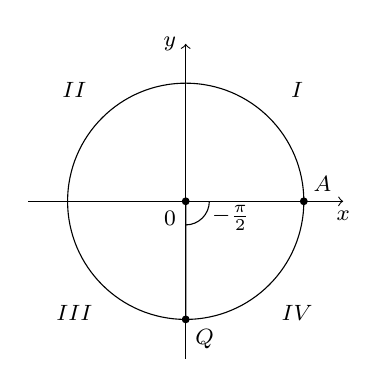
\begin{tikzpicture}[font=\footnotesize]
					\draw[->] (180:2)--(0:2) node[below] {$x$};
					\draw[->] (-90:2)--(90:2) node[left] {$y$};
					\draw (0:0) circle (1.5);
					\fill (0:0) circle (0.05) node[below left] {$0$};
					\node at (45:2) {$I$};
					\node at (135:2) {$II$};
					\node at (225:2) {$III$};
					\node at (-45:2) {$IV$};
					\fill (-90:1.5) circle (0.05) node[ below right ] {$Q$};
					\fill (0:1.5) circle (0.05) node[above right] {$A$};
					\draw (0:0)--(-90:1.5)  (0:0.3) arc (0:-90:0.3);
					\node[right] at (-45:0.3) {$-\frac{\pi}{2}$};
				\end{tikzpicture}
			}			
		\end{itemchoice}
	}
\end{ex}

%%%==============EX_4============%%%
\begin{ex} %[1D1H1-5]
	Các góc có cùng điểm biểu diễn trên đường tròn lượng giác \textbf{ĐÚNG} hay \textbf{SAI}?
	\choiceTF
	{\True $756 ^{\circ}$, $-324 ^{\circ}$}
	{\True $-324 ^{\circ}$, $ 36 ^{\circ}$}
	{$36 ^{\circ}$,$ 216 ^{\circ}$}
	{\True $-\dfrac{41\pi}{7}$, $\dfrac{15\pi}{7}$}
	\loigiai{
		Ta có
		$$	\begin{aligned}
			756 ^{\circ}&=36 ^{\circ}+2\cdot 360 ^{\circ}\\
			-324 ^{\circ}&=36 ^{\circ}-360 ^{\circ}\\
			216 ^{\circ}&=-144 ^{\circ}+ 360 ^{\circ}\\
			-\dfrac{41\pi}{7}&=-\dfrac{42\pi-\pi}{7}=\dfrac{\pi}{7}-6\pi\\
			\dfrac{15\pi}{7}&=\dfrac{\pi+14\pi}{7}=\dfrac{\pi}{7}+2\pi
		\end{aligned}$$
		Nên
		\begin{itemchoice}
			\itemch $756 ^{\circ}$ và $-324 ^{\circ}$ có cùng điểm biểu diễn trên trường tròn lượng giác.
			\itemch  $36^{\circ}$ và $-324 ^{\circ}$ có cùng điểm biểu diễn trên trường tròn lượng giác.
			\itemch $36^{\circ}$ và $216^{\circ}$ không có cùng điểm biểu diễn trên trường tròn lượng giác.
			\itemch $	-\dfrac{41\pi}{7}$ và $\dfrac{15\pi}{7}$ có cùng điểm biểu diễn trên trường tròn lượng giác.
		\end{itemchoice}
	}
	
	
\end{ex}		

\Closesolutionfile{ans}
\indapan{3}{ans/ans1-ds}


\Opensolutionfile{ans}[ans/ans1-KQ]
\caukq
%%%==============BT_1==============%%%
\begin{bt}%[1D1V1-4]
	\immini{	Một cái đồng hồ treo tường có đường kính bằng $60$ cm, ta xem vành ngoài chiếc đồng hồ là một đường tròn với các điểm $A$, $B$, $C$ lần lượt tương ứng với vị trí các số $2$, $9$, $4$.
		Tính độ dài các cung nhỏ $AB$  (kết quả tính theo đơn vị centimét và làm tròn đến hàng phần trăm).}{\begin{tikzpicture}[r/.style={font=\sffamily,
				inner sep=0,
				rotate=-30*\x,
				anchor=north},
			declare function = {hour= 10; minute= 15; second =45;},
			s/.style={even odd rule,
				top color= black,
				bottom color= black,
				middle color=white},scale=0.8]
			\pgfmathsetmacro{\hourhand}{hour}
			\pgfmathsetmacro{\minutehand}{minute}
			\pgfmathsetmacro{\secondhand}{second}
			\shade[s,shading angle=-10] circle (21mm) circle (22mm);
			\shade[s,shading angle=15] circle (22mm) circle (25mm);
			\foreach\x[evaluate={\xf=int(5*\x);}] in{1,...,12}{
				\draw ({30*(3-\x)}:19mm) node[r,anchor=south,scale=0.5,inner sep=1pt] {\xf}
				node[r,scale=1.5,xscale=0.85] at ({30*(3-\x)}:1.8cm)
				{\uppercase\expandafter{\romannumeral\x}};
				\ifodd\x\else\draw (30*\x:18mm-2.5ex)--++(30*\x:-1mm);\fi
			}
			\foreach\x in{1,...,60}{\draw (6*\x:18mm)--++(6*\x:1mm);}
			\draw circle(18mm) circle(19mm) circle(18mm-2.5ex) circle(17mm-2.5ex);
			\begin{scope}[rotate around={-6*(\minutehand):(0,0)}]%\hourhand+
				\fill(0.5mm,0) to[out=90,in=-100] (80:1.2cm) to[in=-80,out=120] (90:1.75cm)
				to[out=-100,in=60] (100:1.2cm) to[in=90,out=-80](-0.5mm,0);
			\end{scope}
			\begin{scope}[rotate around={-30*(\hourhand+\minutehand/60):(0,0)}]
				\fill(0.5mm,0) to[out=90,in=-150] (70:6mm) to[in=-80,out=120] (90:1.4cm)
				to[out=-100,in=60] (110:6mm) to[in=90,out=-30](-0.5mm,0);
			\end{scope}
			\draw[thick,-{Kite[scale=0.8]}] (0,0) -- (90-6*\secondhand:1.8cm); %Seconds
			\filldraw[fill=white]circle (1mm);
			\node at (32:30mm) {$A$};
			\node at (180:30mm) {$B$};
			\node at (-32:30mm) {$C$};
	\end{tikzpicture}}
	\shortans{$78${,}$5$}
	\loigiai{
		Bán kính đường tròn là $R=\dfrac{60}{2}=30 $ (cm).\\[2pt]
		Ta có $\widehat{AOB}=150 ^{\circ}=\dfrac{150\pi}{180}$ rad $=\dfrac{5\pi}{6} $ rad.\\
		Suy ra độ dài cung nhỏ $AB$ là $l_{\wideparen{AB}}=R\cdot \widehat{AOB}=30\cdot \dfrac{5\pi}{6}=25\pi \approx 78{,}54  $ (cm).
	}
\end{bt}

%%%==============BT_2==============%%%
\begin{bt}%[1D1V1-2]
	\immini{Một chiếc đồng hồ có kim giờ và kim phút được cho như trong hình vẽ sau. Xét tia $Ou$ là kim giờ, $Ov$ là kim phút. Xét chiều quay của góc là chiều kim đồng hồ. Số góc lượng giác $(Ou,Ov)$ là bao nhiêu  ( với $k =0$ và số đo tính bằng độ)?}{	\begin{tikzpicture}[r/.style={font=\sffamily,
				inner sep=0,
				rotate=-30*\x,
				anchor=north},
			declare function = {hour= 9; minute= 0; second =45;},
			s/.style={even odd rule,
				top color= black,
				bottom color= black,
				middle color=white},scale=0.8]
			\pgfmathsetmacro{\hourhand}{hour}
			\pgfmathsetmacro{\minutehand}{minute}
			\pgfmathsetmacro{\secondhand}{second}
			\shade[s,shading angle=-10] circle (21mm) circle (22mm);
			\shade[s,shading angle=15] circle (22mm) circle (25mm);
			\foreach\x[evaluate={\xf=int(5*\x);}] in{1,...,12}{
				\draw ({30*(3-\x)}:19mm) node[r,anchor=south,scale=0.5,inner sep=1pt] {\xf}
				node[r,scale=1.5,xscale=0.85] at ({30*(3-\x)}:1.8cm)
				{\uppercase\expandafter{\romannumeral\x}};
				\ifodd\x\else\draw (30*\x:18mm-2.5ex)--++(30*\x:-1mm);\fi
			}
			\foreach\x in{1,...,60}{\draw (6*\x:18mm)--++(6*\x:1mm);}
			\draw circle(18mm) circle(19mm) circle(18mm-2.5ex) circle(17mm-2.5ex);
			\begin{scope}[rotate around={-6*(\minutehand):(0,0)}]%\hourhand+
				\fill(0.5mm,0) to[out=90,in=-100] (80:1.2cm) to[in=-80,out=120] (90:1.75cm)
				to[out=-100,in=60] (100:1.2cm) to[in=90,out=-80](-0.5mm,0);
			\end{scope}
			\begin{scope}[rotate around={-30*(\hourhand+\minutehand/60):(0,0)}]
				\fill(0.5mm,0) to[out=90,in=-150] (70:6mm) to[in=-80,out=120] (90:1.4cm)
				to[out=-100,in=60] (110:6mm) to[in=90,out=-30](-0.5mm,0);
			\end{scope}
			\draw[thick,-{Kite[scale=0.8]}] (0,0) -- (90-6*\secondhand:1.8cm); %Seconds
			\filldraw[fill=white]circle (1mm);
	\end{tikzpicture}}
	
	\shortans{$90$}
	\loigiai{
		Ta có $(Ou,Ov)=90 ^{\circ}+k360 ^{\circ} \,  (k\in \mathbb{Z})$.
	}
\end{bt}

%%%==============BT_3==============%%%
\begin{bt}%[1D1N1-2]
	Đổi số đo góc $\dfrac{2\pi}{5}$ sang độ.
	\shortans{$72$}
	\loigiai{
		Ta có $\dfrac{2\pi}{5}=\dfrac{2\cdot 180 ^{\circ}}{5}=72^0$.
	}
\end{bt}

%%%==============BT_4==============%%%
\begin{bt}%[1D1V1-6]
	Trong $20$ giây bánh xe của xe gắn máy quay được $60$ vòng. Tính độ dài quãng đường xe gắn máy đã đi được trong vòng $3$ phút, biết rằng bán kính bánh xe gắn máy bằng $0{,}65 $ dm (lấy $\pi=3{,}1416$, làm tròn đến hàng đơn vị).
	\shortans{ $2205$}
	\loigiai{
		Ta có
		
		$3$ phút xe đi được $\dfrac{3\times 60}{20} \times 60=540$ vòng.
		
		Độ dài $1$ vòng bằng chu vi bánh xe là $2\pi R=2\times 3{,}1416\times 0{,}65=4{,}08408 $ (dm).
		
		Vậy quãng đường xe đi được là $540\times 4{,}08408=2205{,}4032$ (dm).
	}
\end{bt}

%%%==============BT_5==============%%%
%\begin{bt}%[1D1H1-3]
%	Trên đường tròn với điểm gốc là $A$. Điểm $M$ thuộc đường tròn sao cho cung lượng giác $AM$ có số đo $60 ^{\circ}$. Gọi $N$ là điểm đối xứng với điểm $M$ qua trục $Oy$. Tìm số đo của cung $AN$.
%	\shortans {$120$}
%	\immini{	\loigiai{
%			
%			Ta có $\widehat{AOM}=60 ^{\circ}, \widehat{MON}=60 ^{\circ}$ nên $\widehat{AON}=120 ^{\circ}$.
%			Khi đó số đo cung $AN$ bằng $120 ^{\circ}$.
%	}}{
%		\begin{tikzpicture}[>=stealth,scale=0.75, font=\footnotesize]
%			\draw [->](180:3)--(0:3) node[below] {$x$};
%			\draw [->](-90:3)--(90:3) node[left] {$y$};
%			\draw (0:0) circle (2);
%			\draw (0:2) circle (0.05) node[above right]{$A$};
%			\draw (60:2) circle (0.05) node[above right]{$M$};
%			\draw (120:2) circle (0.05) node[above left]{$N$};
%			\draw (0:0)--(60:2)--(120:2)--cycle;
%			\path (0:0)node[below left]{$0$};
%		\end{tikzpicture}
%	}
%\end{bt}


%%%==============BT_6==============%%%
\begin{bt}%[1D1C1-6]
	Một bánh xe có đường kính kể cả lốp xe là $55$ cm. Nếu xe chạy với tốc độ $50$  km/h thì trong một giây bánh xe quay được bao nhiêu vòng (Kết quả được làm tròn đến hàng phần trăm)?
	\shortans{$8{,}04$}
	\loigiai{
		Tốc độ xe là
		$$\begin{aligned}
			50 \text{ km/h} &= \dfrac{50\cdot100000}{3600}&&   \text{ cm/s}\\
			&= \dfrac{12500}{9}  && \text{ cm/s.}
		\end{aligned}$$
		Mỗi vòng bánh xe có chiều dài là $2\pi R=2\pi \cdot \dfrac{55}{2}=55\pi$ (cm).\\[2pt]
		Vậy mỗi giây thì bánh xe lăn được số vòng là $\dfrac{12500}{9}:(55\pi)\approx 8{,}04$ (vòng).
	}
\end{bt}
\Closesolutionfile{ans}
\indapan{6}{ans/ans1-KQ}
\newpage

\subsection{Đề 2}
\Opensolutionfile{ans}[ans/ans2]
\caulc
%%%==============EX_1============%%%
\begin{ex}%[1D1N1-2]
	Cung có số đo $250^\circ$ thì có số đo theo đơn vị radian là
	\choice
	{$\dfrac{25\pi}{12}$}
	{\True $\dfrac{25\pi}{18}$}
	{$\dfrac{25\pi}{9}$}
	{$\dfrac{35\pi}{18}$}
	\loigiai{
		Ta có $250^\circ=\dfrac{250 \cdot \pi}{180}=\dfrac{25\pi}{18}$.
	}
\end{ex}
%%%==============EX_2============%%%
\begin{ex}%[1D1N1-2]
	Đổi sang radian góc có số đo $108^\circ$ ta được
	\choice
	{$\dfrac{\pi}{4}$}
	{$\dfrac{\pi}{10}$}
	{$\dfrac{3\pi}{2}$}
	{\True $\dfrac{3\pi}{5}$}
	\loigiai{
		Ta có $1^\circ=\dfrac{\pi}{180}$ nên $108^\circ=\dfrac{108\pi}{180}$ $=\dfrac{3\pi}{5}$.
	}
\end{ex}
%%%==============EX_3============%%%
\begin{ex}%[1D1N1-1]
	Tìm mệnh đề đúng.
	\choice
	{$\pi$ rad $=\left(\dfrac{180}{\pi} \right)$}
	{$\pi$ rad$=1^\circ$}
	{$\pi$ rad $=60^\circ$}
	{\True $\pi$ rad $=180^\circ$}
	\loigiai{
	}
\end{ex}
%%%==============EX_4============%%%
\begin{ex}%[1D1N1-2]
	Số đo radian của góc $135^\circ$ là
	\choice
	{$\dfrac{\pi}{6}$}
	{\True $\dfrac{3\pi}{4}$}
	{$\dfrac{2\pi}{3}$}
	{$\dfrac{\pi}{2}$}
	\loigiai{
		Sử dụng máy tính bỏ túi ta tính được $135^\circ=\dfrac{3\pi}{4}$.
	}
\end{ex}

%%%==============EX_5============%%%
\begin{ex}%[1D1N1-2]
	Góc có số đo $-\dfrac{3\pi}{16}$ có số đo theo độ là
	\choice
	{$33^{\circ} 45'$}
	{$-29^{\circ} 30'$}
	{$-32^{\circ} 55'$}
	{\True $-33^{\circ} 45'$}
	\loigiai{
		Vì $1$ rad $=\left(\dfrac{180}{\pi} \right)^{\circ}$ nên $\dfrac{-3\pi}{16}=\left(\dfrac{-3\pi}{16} \cdot \dfrac{180}{\pi} \right)^{\circ}=\left(\dfrac{-135}{4} \right)^{\circ}=-33,75^{\circ}=-33^{\circ} 45'$.
	}
\end{ex}
%%%==============EX_6============%%%
\begin{ex}%[1D1N1-2]
	Nếu một góc có số đo $\dfrac{5\pi}{12}$ rad thì số đo của góc đó khi đổi sang đơn vị độ, phút, giây là
	\choice
	{$45^\circ$}
	{\True $75^\circ$}
	{$55^\circ$}
	{$65^\circ$}
	\loigiai{
		Ta có $1$ rad $=\left(\dfrac{180}{\pi} \right)^\circ \Rightarrow \dfrac{5\pi}{12}$  rad $=\left(\dfrac{180}{\pi}\cdot \dfrac{5\pi}{12} \right)^\circ=75^\circ$.
	}
\end{ex}



%%%==============EX_7============%%%
\begin{ex}%[1D1H1-4]
	Tính bán kính $R$ của đường tròn biết rằng cung có số đo $\dfrac{5}{3}$ rad dài $24$ cm.
	\choice
	{$R=4{,}0$ cm}
	{$R=4{,}6$ cm}
	{\True $R=14{,}4$ cm}
	{$1{,}6$ cm}
	\loigiai{
		Áp dụng công thức $l=\alpha \cdot R$ ta có $R=\dfrac{l}{\alpha}=\dfrac{24}{\left(\dfrac{5}{3} \right)}=14{,}4$ (cm).
	}
\end{ex}
%%%==============EX_8============%%%
\begin{ex}%[1D1N1-4]
	Cho đường tròn có bán kính $6$ cm. Tìm số đo (rad) của cung có độ dài $3$ cm.
	\choice
	{$1$}
	{\True $0{,}5$}
	{$2$}
	{$3$}
	\loigiai{
		Đường tròn có bán kính $R=6$ cm và cung có độ dài $l=3$ cm.\\
		Số đo của cung là $\alpha=\dfrac{l}{R}=\dfrac{1}{2}$ (rad).
	}
\end{ex}

%%%==============EX_9============%%%
\begin{ex}%[1D1N1-4]
	Một đường tròn có bán kính $R=12$ cm. Tính độ dài của cung $60^\circ$ trên đường tròn gần bằng
	\choice
	{$2$ cm}
	{$4$ cm}
	{$6{,}28$ cm}
	{\True $12{,}56$ cm}
	\loigiai{
		Ta có $60^\circ$ tương ứng với góc $\dfrac{\pi}{3}$ rad.
		
		Do đó độ dài cung tròn là $l=R\alpha=12\cdot \dfrac{\pi}{3}=4\pi=12{,}56$ cm.
	}
\end{ex}


%%%==============EX_10============%%%
\begin{ex}%[1D1C1-6]
	Bánh xe đạp có đường kính $55$ cm (kể cả lốp). Nếu chạy với vận tốc $40$ km/h thì trong $25$ s bánh xe quay được số vòng gần bằng với kết quả nào dưới đây?
	\choice
	{$52$}
	{\True $161$}
	{$322$}
	{$200$}
	\loigiai{
		Ta có $\heva{&r=\dfrac{55}{2} \text{ cm} = \dfrac{0,55}{2} \text{ m}\\ & v = 40 \text{ km/h} = \dfrac{40000}{3600} \text{ m/s}}$ \\
		Gọi $l$ là quãng đường đi được trong $25$ giây.\\
		Gọi $x$ là số vòng bánh xe quay được trong $25$ giây.\\
		Khi đó $l=2\pi\cdot r \cdot x$\\
		Mà $l=\dfrac{25\cdot40000}{3600}=\dfrac{2500}{9}$ suy ra $x=\dfrac{l}{2\pi \cdot r}=160{,}7\approx 161$ (vòng).
	}
\end{ex}
%%%==============EX_11============%%%
\begin{ex}%[1D1V1-6]
	Kim giờ của đồng hồ dài $8$ cm, kim phút dài $10$ cm. Tổng quãng đường mũi kim phút, kim giờ đi được trong $30$ phút bằng
	\choice
	{$\dfrac{25}{3} \pi$}
	{$\dfrac{37}{3} \pi$}
	{$\dfrac{20}{3} \pi$}
	{\True $\dfrac{32}{3} \pi$}
	\loigiai{
		Trong $30$ phút, kim phút quay được một góc là $\pi$ rad.\\
		Quãng đường kim phút đi được là $S_1=\pi \cdot 10=10\pi$ (cm).\\
		Trong $30$ phút kim giờ quay được một góc là $\dfrac{\pi}{12}$ rad.\\
		Quãng đường kim giờ đi được là $S_2=\dfrac{\pi}{12} \cdot 8=\dfrac{2\pi}{3}$ (cm).\\
		Vậy tổng quãng đường cần tìm là $S=S_1+S_2=10\pi+\dfrac{2\pi}{3}=\dfrac{32}{3} \pi$ (cm).
	}
\end{ex}

%%%==============EX_12============%%%
\begin{ex}%[1D1H1-3]
	Cho góc lượng giác $\left(Ou,Ov\right)$ có số đo bằng $\dfrac{\pi}{6}$ rad. Trong các số sau, số đo của góc lượng giác có cùng tia đầu, tia cuối với góc lượng giác đã cho là
	\choice
	{$\dfrac{7\pi}{6}$}
	{\True $\dfrac{-11\pi}{6}$}
	{$\dfrac{19\pi}{6}$}
	{$\dfrac{-25\pi}{6}$}
	\loigiai{
		Ta có $\dfrac{7\pi}{6}=\dfrac{\pi}{6}+\pi$; $\dfrac{-11\pi}{6}=\dfrac{\pi}{6}-2\pi$; $\dfrac{19\pi}{6}=\dfrac{\pi}{6}+3\pi$; $\dfrac{-25\pi}{6}=\dfrac{\pi}{6}-\dfrac{13\pi}{3}$.
		
		Do góc lượng giác có số đo $\alpha$ rad thì mọi góc lượng giác có cùng tia đầu, tia cuối với nó có số đo dạng $\alpha+k2\pi$ rad $\left(k\in \mathbb{Z}\right)$.
		
		Nên với góc lượng giác $\left(Ou,Ov\right)$ có số đo bằng $\dfrac{\pi}{6}$ rad thì trong các góc lượng giác trên góc lượng giác có cùng tia đầu và tia cuối với nó là $\dfrac{-11\pi}{6}$.
	}
\end{ex}
\Closesolutionfile{ans}
\indapan{6}{ans/ans2}

\cauds
\Opensolutionfile{ans}[ans/ans2-ds]


%%%==============EX_1============%%%
\begin{ex}%[1D1N1-2]
	Đổi số đo của các góc sang độ. Khẳng định sau đây \textbf{ĐÚNG} hay \textbf{SAI} ?
	\choiceTF
	{\True $\dfrac{3\pi}{4}$ rad $= 135 ^{\circ}$}
	{\True $-\dfrac{\pi}{360}$ rad $=-0,5 ^{\circ}$}
	{$\dfrac{31\pi}{2}$ rad $ =27 ^{\circ}$}
	{\True $-4$ rad $\approx-229{,}18 ^{\circ}$}
	\loigiai{
		\begin{itemchoice}
			\itemch $\dfrac{3\pi}{4}$ rad$ =\left(\dfrac{3\pi}{4} \cdot \dfrac{180}{\pi} \right) ^{\circ}=135 ^{\circ}$.
			\itemch $-\dfrac{\pi}{360}$ rad$ =\left(-\dfrac{\pi}{360} \cdot \dfrac{180}{\pi} \right) ^{\circ}=-0,5 ^{\circ}$.
			\itemch 	$\dfrac{31\pi}{2}$ rad$ =\left(\dfrac{31\pi}{2} \cdot \dfrac{180}{\pi} \right) ^{\circ}=2790 ^{\circ}$.
			\itemch 	$-4$ rad $=\left(-4\cdot \dfrac{180}{\pi} \right) ^{\circ}=\left(-\dfrac{720}{\pi} \right) ^{\circ} \approx-229,18 ^{\circ}$.
		\end{itemchoice}
	}
\end{ex}


%%%==============EX_2============%%%
\begin{ex}%[1D1H1-5]
	\immini{Biểu diễn góc lượng giác trên đường tròn lượng giác. Các mệnh đề sau \textbf{ĐÚNG} hay \textbf{SAI} ?
		\choiceTF
		{$36 ^{\circ}+k360 ^{\circ}, \, k\in \mathbb{Z}$ là điểm $M$ thuộc góc phần tư thứ $II$}
		{\True $-60 ^{\circ}+k180 ^{\circ},\, k\in \mathbb{Z}$ là các điểm $M_1$, $M_2$ thuộc góc phần tư thứ $II$ và $IV$}
		{$-\dfrac{\pi}{4}+k2\pi$, $  k\in \mathbb{Z}$ là $M$ thuộc góc phần tư thứ $III$}
		{\True $-\dfrac{\pi}{6}+k\dfrac{\pi}{2}$, $ k\in \mathbb{Z}$ là bốn điểm  $M$,  $N$, $P$, $Q$ thuộc góc phần tư thứ $I$, $II$, $III$, $IV$}}{
		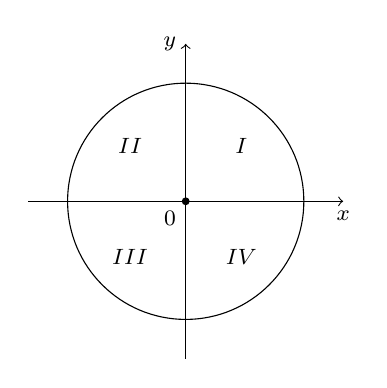
\begin{tikzpicture}[font=\footnotesize]
			\draw[->] (180:2)--(0:2) node[below] {$x$};
			\draw[->] (-90:2)--(90:2) node[left] {$y$};
			\draw (0:0) circle (1.5);
			\fill (0:0) circle (0.05) node[below left] {$0$};
			\node at (45:1) {$I$};
			\node at (135:1) {$II$};
			\node at (225:1) {$III$};
			\node at (-45:1) {$IV$};
		\end{tikzpicture}
	}
	\loigiai{
		\begin{itemchoice}
			\itemch 	\immini{Xét góc lượng giác $k360 ^{\circ}$, dù $k$ là số chẵn hay số lẻ thì góc này cũng có điểm biểu diễn là điểm $A$ (điểm gốc trên đường tròn lượng giác).
				
				Vì vậy, góc lượng giác $36 ^{\circ}+k360 ^{\circ}$ có điểm biểu diễn là điểm $M$ thuộc góc phần tư thứ $I$ của đường tròn lượng giác và $\widehat{AOM}=36 ^{\circ}$.}
			{
				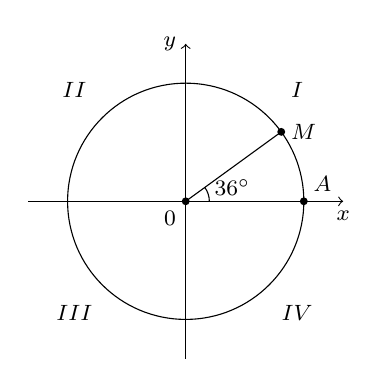
\begin{tikzpicture}[font=\footnotesize]
					\draw[->] (180:2)--(0:2) node[below] {$x$};
					\draw[->] (-90:2)--(90:2) node[left] {$y$};
					\draw (0:0) circle (1.5);
					\fill (0:0) circle (0.05) node[below left] {$0$};
					\node at (45:2) {$I$};
					\node at (135:2) {$II$};
					\node at (225:2) {$III$};
					\node at (-45:2) {$IV$};
					\fill (36:1.5) circle (0.05) node[right] {$M$};
					\fill (0:1.5) circle (0.05) node[above right] {$A$};
					%\draw (0:0.3) arc (36:0.3);
					\draw (0:0)--(36:1.5)  (0:0.3) arc (0:36:0.3) node[right] {$36^\circ$};
				\end{tikzpicture}
			}
			
			\itemch 	\immini{Xét góc lượng giác $k180 ^{\circ}$. Nếu $k$ chẵn thì góc này có điểm biểu diễn là $A(1;0)$, nếu $k$ lẻ thì góc này có điểm biểu diễn là điểm $B(-1;0)$.
				
				Vì vậy, $-60 ^{\circ}+k180 ^{\circ}$ có các điểm biểu diễn là $M_1$ và $M_2$ như hình vẽ bên.}
			{
				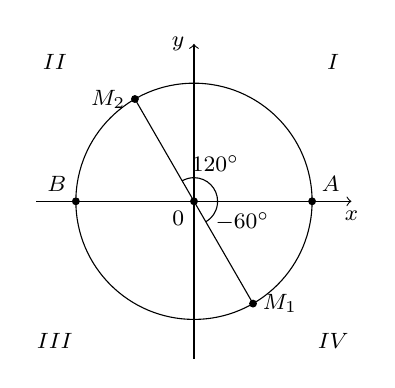
\begin{tikzpicture}[font=\footnotesize]
					\draw[->] (180:2)--(0:2) node[below] {$x$};
					\draw[->] (-90:2)--(90:2) node[left] {$y$};
					\draw (0:0) circle (1.5);
					\fill (0:0) circle (0.05) node[below left] {$0$};
					\node at (45:2.5) {$I$};
					\node at (135:2.5) {$II$};
					\node at (225:2.5) {$III$};
					\node at (-45:2.5) {$IV$};
					\fill (-60:1.5) circle (0.05) node[right] {$M_1$};
					\fill (120:1.5) circle (0.05) node[left] {$M_2$};
					\fill (0:1.5) circle (0.05) node[above right] {$A$};
					\fill (180:1.5) circle (0.05) node[above left] {$B$};
					%\draw (0:0.3) arc (36:0.3);
					\draw (0:0)--(-60:1.5)  (0:0.3) arc (0:-60:0.3) node[right] {$-60^\circ$};
					\draw(0:0)--(120:1.5)  (0:0.3) arc (0:120:0.3) node[above right] {$120^\circ$};
				\end{tikzpicture}
			}
			
			\itemch \immini{ Ta biết góc lượng giác $k2\pi$ luôn có điểm biểu diễn là $A(1;0)$, vì vậy góc lượng giác $-\dfrac{\pi}{4}+k2\pi$ có điểm biểu diễn là $M$ thuộc góc phần tư thứ IV và thoả mãn $\widehat{AOM}=\dfrac{\pi}{4}$.}
			{
				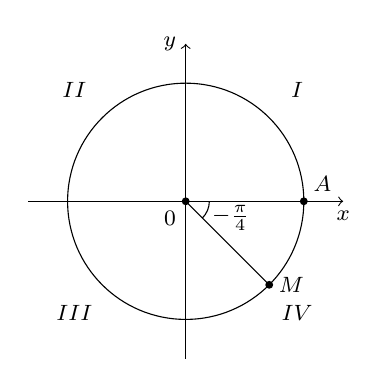
\begin{tikzpicture}[font=\footnotesize]
					\draw[->] (180:2)--(0:2) node[below] {$x$};
					\draw[->] (-90:2)--(90:2) node[left] {$y$};
					\draw (0:0) circle (1.5);
					\fill (0:0) circle (0.05) node[below left] {$0$};
					\node at (45:2) {$I$};
					\node at (135:2) {$II$};
					\node at (225:2) {$III$};
					\node at (-45:2) {$IV$};
					\fill (-45:1.5) circle (0.05) node[right] {$M$};
					\fill (0:1.5) circle (0.05) node[above right] {$A$};
					%\draw (0:0.3) arc (36:0.3);
					\draw (0:0)--(-45:1.5)  (0:0.3) arc (0:-45:0.3) node[right] {$-\frac{\pi}{4}$};
				\end{tikzpicture}
			}
			
			
			\itemch 	\immini{	Xét góc lượng giác $k\dfrac{\pi}{2}$. Khi $k=0$ thì $k\dfrac{\pi}{2}=0$, góc này có điểm biểu diễn là điểm $A(1;0)$. Khi $k=1$ thì $k\dfrac{\pi}{2}=\dfrac{\pi}{2}$, góc này có điểm biểu diễn là điểm $C(0;1)$. 
				
				Khi $k=2$ thì $k\dfrac{\pi}{2}=\pi$, góc này có điểm biểu diễn là điểm $B(-1;0)$.
				
				Khi $k=3$ thì $k\dfrac{\pi}{2}=\dfrac{3\pi}{2}$, góc này có điểm biểu diễn là điểm $D(0;-1)$. Nếu $k=4,5,6,\ldots$ thì ta thấy rằng các điểm biểu diễn có được vẫn là sự lặp lại của $A,B,C,D$.
				
				Vì vậy điểm biểu diễn của $-\dfrac{\pi}{6}+k\dfrac{\pi}{2}$ là bốn điểm $M,N,P,Q$ trên đường tròn lượng giác (xem hình vẽ trên).}	{
				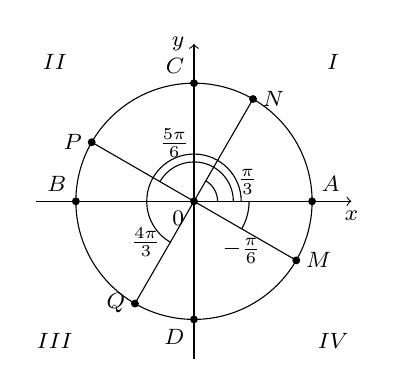
\begin{tikzpicture}[font=\footnotesize]
					\draw[->] (180:2)--(0:2) node[below] {$x$};
					\draw[->] (-90:2)--(90:2) node[left] {$y$};
					\draw (0:0) circle (1.5);
					\fill (0:0) circle (0.05) node[below left] {$0$};
					\node at (45:2.5) {$I$};
					\node at (135:2.5) {$II$};
					\node at (225:2.5) {$III$};
					\node at (-45:2.5) {$IV$};
					\fill (60:1.5) circle (0.05) node[right] {$N$};
					\fill (-30:1.5) circle (0.05) node[right] {$M$};
					\fill (150:1.5) circle (0.05) node[left] {$P$};
					\fill (240:1.5) circle (0.05) node[left] {$Q$};
					\fill (0:1.5) circle (0.05) node[above right] {$A$};
					\fill (180:1.5) circle (0.05) node[above left] {$B$};
					\fill (90:1.5) circle (0.05) node[above left] {$C$};
					\fill (-90:1.5) circle (0.05) node[below left] {$D$};
					\draw (0:0)--(60:1.5)  (0:0.3) arc (0:60:0.3) ;
					\node[right] at (30:0.5) {$\frac{\pi}{3}$};
					\draw(0:0)--(150:1.5)  (0:0.5) arc (0:150:0.5); \node[above] at (120:0.5) {$\frac{5\pi}{6}$};
					\draw(0:0)--(240:1.5)  (0:0.6) arc (0:240:0.6) node[ left] {$\frac{4\pi}{3}$};
					\draw(0:0)--(-30:1.5)  (0:0.7) arc (0:-30:0.7) node[below] {$-\frac{\pi}{6}$};
				\end{tikzpicture}
			}
		\end{itemchoice}
	}			
\end{ex}

%%%==============EX_3============%%%
\begin{ex}%[1D1H1-5]
	Các cặp góc  sau có cùng điểm biểu diễn trên đường tròn lượng giác \textbf{ĐÚNG} hay \textbf{SAI} ?
	\choiceTF
	{\True $1127 ^{\circ}{,}-313 ^{\circ}$}
	{$1127 ^{\circ}{,}-674$}
	{\True $\dfrac{61\pi}{5}{,}-\dfrac{19\pi}{5}$}
	{$\dfrac{61\pi}{5}{,}-\dfrac{23\pi}{4}$}
	\loigiai{
		\begin{itemchoice}
			\itemch 	Ta có $1127 ^{\circ}=47 ^{\circ}+3\cdot360 ^{\circ}$; $ -313 ^{\circ}=47 ^{\circ}-360 ^{\circ}$.\\
			Vì vậy các góc lượng giác $1127 ^{\circ}{,}-313 ^{\circ}$ có cùng một điểm biểu diễn và điểm này trùng với điểm biểu diễn của góc $47 ^{\circ}$ trên đường tròn lượng giác.
			\itemch Ta có $-674 ^{\circ}=46 ^{\circ}-2\cdot 360 ^{\circ}$ nên không trùng điểm biểu diễn với góc $1127^\circ$.
			\itemch  		Ta có: $\dfrac{61\pi}{5}=\dfrac{\pi}{5}+6\cdot2\pi$ ;  $-\dfrac{19\pi}{5}=\dfrac{\pi}{5}-2\cdot 2\pi$.\\
			Vì vậy các góc lượng giác $\dfrac{61\pi}{5}$ , $-\dfrac{19\pi}{5}$ có cùng một điểm biểu diễn và điểm này trùng với điểm biểu diễn của góc $\dfrac{\pi}{5}$ trên đường tròn lượng giác.
			\itemch Ta có $-\dfrac{23\pi}{4}=\dfrac{\pi}{4}-3\cdot 2\pi$  nên không trùng điểm biểu diễn với góc $\dfrac{61\pi}{5}$.
		\end{itemchoice}
	}	
\end{ex}		



%%%==============EX_4============%%%
\begin{ex}%[1D1H1-6]
	\immini{Trong hình vẽ bên, ta xem hình ảnh đường tròn trên một bánh lái tàu thuỷ tương ứng với một đường tròn lượng giác. Các mệnh đề sau \textbf{ĐÚNG} hay \textbf{SAI} ?
		\choiceTF
		{\True Công thức tổng quát biểu diễn góc lượng giác $(OA,OB)$ theo đơn vị radian: $(OA,OB)=\dfrac{\pi}{4}+k2\pi \, (k\in \mathbb{Z})$}
		{Công thức tổng quát chỉ ra góc lượng giác tương ứng với bốn điểm biểu diễn là $A$, $C$, $E$, $G$ theo đơn vị radian là $k\dfrac{\pi}{3} (k\in \mathbb{Z})$}
		{\True Công thức tổng quát chỉ ra góc lượng giác tương ứng với hai điểm biểu diễn là $A$, $E$ theo đơn vị độ là $k180 ^{\circ} (k\in \mathbb{Z})$}
		{Công thức tổng quát biểu diễn góc lượng giác $(OA,OC)+(OC,OH)$ theo đơn vị radian là	$\dfrac{\pi}{4}+k2\pi (k\in \mathbb{Z})$}
	}
	{
					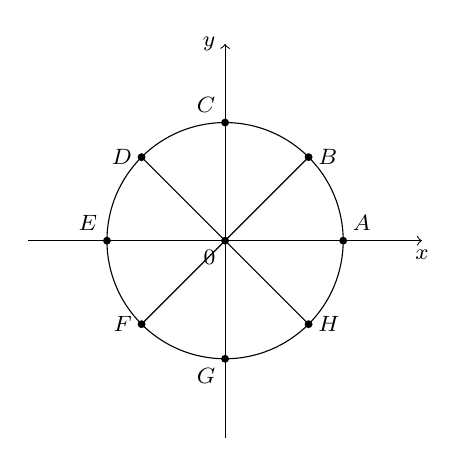
\begin{tikzpicture}[font=\footnotesize]
			\draw[->] (180:2.5)--(0:2.5) node[below] {$x$};
			\draw[->] (-90:2.5)--(90:2.5) node[left] {$y$};
			\draw (0:0) circle (1.5);
			\fill (0:0) circle (0.05) node[below left] {$0$};
			\fill (45:1.5) circle (0.05) node[right] {$B$};
			\fill (-45:1.5) circle (0.05) node[right] {$H$};
			\fill (135:1.5) circle (0.05) node[left] {$D$};
			\fill (225:1.5) circle (0.05) node[left] {$F$};
			\fill (0:1.5) circle (0.05) node[above right] {$A$};
			\fill (180:1.5) circle (0.05) node[above left] {$E$};
			\fill (90:1.5) circle (0.05) node[above left] {$C$};
			\fill (-90:1.5) circle (0.05) node[below left] {$G$};
			\draw (0:0)--(45:1.5);
			\draw(0:0)--(135:1.5)  ;
			\draw(0:0)--(225:1.5) ;
			\draw(0:0)--(-45:1.5) ;
		\end{tikzpicture}}
	\loigiai{
		\begin{itemchoice}
			\itemch Ta có $(OA,OB)=\dfrac{\pi}{4}+k2\pi \, (k\in \mathbb{Z})$.
			\itemch 	Ta thấy $A$, $C $, $E$, $G$ lần lượt biểu diễn cho các góc lượng giác $0$ rad, $\dfrac{\pi}{2}$ rad, $\pi$ rad, $\dfrac{3\pi}{2}$ rad, $2\pi$ rad, $\dfrac{5\pi}{2}$ rad, $\ldots$ Tất cả các góc này theo thứ tự chênh lệch nhau $\dfrac{\pi}{2}$ rad. Vì vậy công thức duy nhất biểu diễn cho các góc lượng giác ấy là $k\dfrac{\pi}{2}\,  (k\in \mathbb{Z})$.
			\itemch Ta thấy hai điểm $A,E$ lần lượt biểu diễn cho các góc lượng giác $0 ^{\circ}$, $180 ^{\circ}$, $360 ^{\circ}$, $540 ^{\circ}, \ldots$ Tất cả các góc này theo thứ tự chênh lệch nhau $180 ^{\circ}$. Vì vậy công thức duy nhất biểu diễn cho các góc lượng giác ấy là $k180 ^{\circ}\, (k\in \mathbb{Z})$.
			\itemch Theo hệ thức Sa-lơ, ta có
			\[\begin{array}{l} {(OA,OB)+(OB,OC)=(OA,OC)=\dfrac{\pi}{2}+k2\pi \, (k\in \mathbb{Z}).} \\ {(OA,OC)+(OC,OH)=(OA,OH)=-\dfrac{\pi}{4}+k2\pi \, (k\in \mathbb{Z}).} \end{array}
			\]
		\end{itemchoice}
	}
\end{ex}



\Closesolutionfile{ans}
\indapan{3}{ans/ans2-ds}

\Opensolutionfile{ans}[ans/ans2-KQ]
\caukq
%%%==============BT_1==============%%%
\begin{bt}%[1D1H1-4]
	\immini{
		Một cái đồng hồ treo tường có đường kính bằng $60$ cm, ta xem vành ngoài chiếc đồng hồ là một đường tròn với các điểm $A$, $B$, $C$ lần lượt tương ứng với vị trí các số $2$, $ 9$, $4$.
		Tính độ dài các cung nhỏ $AC$ (kết quả tính theo đơn vị centimét và làm tròn đến hàng phần chục).
	}{\begin{tikzpicture}[r/.style={font=\sffamily,
				inner sep=0,
				rotate=-30*\x,
				anchor=north},
			declare function = {hour= 5; minute= 20; second =45;},
			s/.style={even odd rule,
				top color= black,
				bottom color= black,
				middle color=white},scale=0.8]
			\pgfmathsetmacro{\hourhand}{hour}
			\pgfmathsetmacro{\minutehand}{minute}
			\pgfmathsetmacro{\secondhand}{second}
			\shade[s,shading angle=-10] circle (21mm) circle (22mm);
			\shade[s,shading angle=15] circle (22mm) circle (25mm);
			\foreach\x[evaluate={\xf=int(5*\x);}] in{1,...,12}{
				\draw ({30*(3-\x)}:19mm) node[r,anchor=south,scale=0.5,inner sep=1pt] {\xf}
				node[r,scale=1.5,xscale=0.85] at ({30*(3-\x)}:1.8cm)
				{\uppercase\expandafter{\romannumeral\x}};
				\ifodd\x\else\draw (30*\x:18mm-2.5ex)--++(30*\x:-1mm);\fi
			}
			\foreach\x in{1,...,60}{\draw (6*\x:18mm)--++(6*\x:1mm);}
			\draw circle(18mm) circle(19mm) circle(18mm-2.5ex) circle(17mm-2.5ex);
			\begin{scope}[rotate around={-6*(\minutehand):(0,0)}]%\hourhand+
				\fill(0.5mm,0) to[out=90,in=-100] (80:1.2cm) to[in=-80,out=120] (90:1.75cm)
				to[out=-100,in=60] (100:1.2cm) to[in=90,out=-80](-0.5mm,0);
			\end{scope}
			\begin{scope}[rotate around={-30*(\hourhand+\minutehand/60):(0,0)}]
				\fill(0.5mm,0) to[out=90,in=-150] (70:6mm) to[in=-80,out=120] (90:1.4cm)
				to[out=-100,in=60] (110:6mm) to[in=90,out=-30](-0.5mm,0);
			\end{scope}
			\draw[thick,-{Kite[scale=0.8]}] (0,0) -- (90-6*\secondhand:1.8cm); %Seconds
			\filldraw[fill=white]circle (1mm);
			\node at (32:30mm) {$A$};
			\node at (180:30mm) {$B$};
			\node at (-32:30mm) {$C$};
	\end{tikzpicture}}
	\shortans{$31,4$}
	\loigiai{
		Bán kính đường tròn là $R=\dfrac{60}{2}=30$ cm.\\
		Ta có
		$\widehat{AOC}=60 ^{\circ}=\dfrac{60\pi}{180}$ rad $=\dfrac{\pi}{3}$ rad.\\
		Suy ra độ dài cung nhỏ $AC$ là
		$l_{\widehat{AC}}=R\cdot \widehat{AOC}=30\cdot \dfrac{\pi}{3}=10\pi \approx 31{,}42 \text{ (cm).}$
	}
\end{bt}

%%%==============BT_2==============%%%
\begin{bt}%[1D1H1-3]
	\immini{
		Một chiếc đồng hồ có kim giờ và kim phút được cho như trong hình vẽ sau. Xét tia $Ou$ là kim giờ, $Ov$ là kim phút. Xét chiều quay của góc là chiều kim đồng hồ. Số góc lượng giác $(Ou,Ov)$ là (với $k =0$ và số đo tính bằng độ)?}{\begin{tikzpicture}[r/.style={font=\sffamily,
				inner sep=0,
				rotate=-30*\x,
				anchor=north},
			declare function = {hour= 4; minute= 0; second =0;},
			s/.style={even odd rule,
				top color= black,
				bottom color= black,
				middle color=white},scale=0.8]
			\pgfmathsetmacro{\hourhand}{hour}
			\pgfmathsetmacro{\minutehand}{minute}
			\pgfmathsetmacro{\secondhand}{second}
			\shade[s,shading angle=-10] circle (21mm) circle (22mm);
			\shade[s,shading angle=15] circle (22mm) circle (25mm);
			\foreach\x[evaluate={\xf=int(5*\x);}] in{1,...,12}{
				\draw ({30*(3-\x)}:19mm) node[r,anchor=south,scale=0.5,inner sep=1pt] {\xf}
				node[r,scale=1.5,xscale=0.85] at ({30*(3-\x)}:1.8cm)
				{\uppercase\expandafter{\romannumeral\x}};
				\ifodd\x\else\draw (30*\x:18mm-2.5ex)--++(30*\x:-1mm);\fi
			}
			\foreach\x in{1,...,60}{\draw (6*\x:18mm)--++(6*\x:1mm);}
			\draw circle(18mm) circle(19mm) circle(18mm-2.5ex) circle(17mm-2.5ex);
			\begin{scope}[rotate around={-6*(\minutehand):(0,0)}]%\hourhand+
				\fill(0.5mm,0) to[out=90,in=-100] (80:1.2cm) to[in=-80,out=120] (90:1.75cm)
				to[out=-100,in=60] (100:1.2cm) to[in=90,out=-80](-0.5mm,0);
			\end{scope}
			\begin{scope}[rotate around={-30*(\hourhand+\minutehand/60):(0,0)}]
				\fill(0.5mm,0) to[out=90,in=-150] (70:6mm) to[in=-80,out=120] (90:1.4cm)
				to[out=-100,in=60] (110:6mm) to[in=90,out=-30](-0.5mm,0);
			\end{scope}
			\draw[thick,-{Kite[scale=0.8]}] (0,0) -- (90-6*\secondhand:1.8cm); %Seconds
			\filldraw[fill=white]circle (1mm);
	\end{tikzpicture}}
	
	\shortans{$240$}
	\loigiai{
		Ta có $(Ou,Ov)=240 ^{\circ}+k360 ^{\circ} (k\in \mathbb{Z})$.	Với $k=0 \Rightarrow (Ou,Ov)=240 ^{\circ}$.
	}
\end{bt}

%%%==============BT_3==============%%%
\begin{bt}%[1D1V1-3]
	\immini{	Cho hình vuông $ABCD$ có tâm $O$ và một trục $(i)$ đi qua $O$. Xác định số đo góc giữa tia $OA$ với trục $(i)$ biết trục $(i)$ đi qua trung điểm I của cạnh $AB$.}{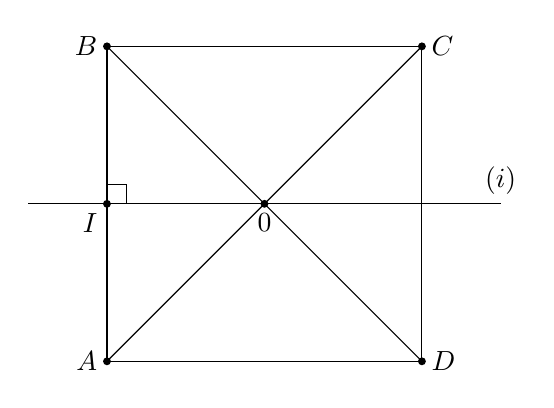
\begin{tikzpicture}
			\draw (0,0)--(4,0)--(4,4)--(0,4)--cycle;
			\draw (0,2)--(0,2.25)--(0.25,2.25)--(0.25,2)--cycle;
			\draw (0,0)--(4,4) (4,0)--(0,4);
			\draw (-1,2)--(5,2) node[above] {$(i)$};
			\fill  (2,2) circle (0.05) node[below] {$0$};
			\fill  (0,0) circle (0.05) node[left] {$A$};
			\fill  (0,4) circle (0.05) node[left] {$B$};
			\fill  (4,0) circle (0.05) node[right] {$D$};
			\fill  (4,4) circle (0.05) node[right] {$C$};
			\fill  (0,2) circle (0.05) node[below left] {$I$};
	\end{tikzpicture}}
	\shortans{$45$}
	\loigiai{
		
		Ta có
		\begin{itemize}
			\item$\widehat{AOB}=90 ^{\circ}$, tam giác $AOB$ vuông cân tại $O$.
			\item 	$(i)$ đi qua trung điểm $I$ của $AB$ nên  $(i)\perp AB$, $(i)$ là đường phân giác của $\widehat{AOB}$.
			\item $(\overrightarrow{OA};(i))=45^\circ$.
		\end{itemize}
	}
\end{bt}

%%%==============BT_4==============%%%
\begin{bt}%[1D1V1-6]
	Một đồng hồ treo tường, kim giờ dài $10,57$ cm và kim phút dài $13,34$ cm. Trong $30$ phút mũi kim giờ vạch lên cung tròn có độ dài bằng bao nhiêu? (làm tròn đến hàng phần trăm).
	\shortans{ $2{,}77$}
	\loigiai{
		Ta có $6$ giờ thì kim giờ vạch lên $1$ cung có số đo $\pi$ nên $30$ phút kim giờ vạch lên $1$ cung có số đo là $\dfrac{1}{12} \pi$.\\
		Suy ra độ dài cung tròn mà nó vạch lên là $l=R\alpha=10{,}57\times \dfrac{3{,}14}{12} \approx 2{,}77$ (cm).
	}
\end{bt}

%%%==============BT_5==============%%%
\begin{bt}
	Một bánh xe có $72$ răng. Số đo góc mà bánh xe đã quay được khi di chuyển $10$ răng là bao nhiêu?
	
	\shortans{$50$}
	\loigiai{
		Ta có $1$ bánh răng tương ứng với $\dfrac{360 ^{\circ}}{72}=5 ^{\circ} \Rightarrow 10$ bánh răng là $50 ^{\circ}$.
	}
\end{bt}

%%%==============BT_6==============%%%
\begin{bt}%[1D1N1-2]
	Đổi số đo của góc $-78 ^{\circ}$ sang radian ( làm tròn đến hàng phần chục).
	\shortans{$-1{,}4$}
	\loigiai{
		\[-78 ^{\circ}=\dfrac{-78^\circ\pi}{180^\circ}=\dfrac{-13\pi}{30} \approx -1{,}4 \text{  rad}.
		\]
	}
\end{bt}
\Closesolutionfile{ans}
\indapan{6}{ans/ans2-KQ}
